\chapter{Test with two free parameters for the Underlying Events}
\label{appendix:test}

Here are reported all the distributions obtained by the test on two parameters:
\begin{itemize}
	\item[--] \texttt{MultipartonInteractions:pT0Ref}
	\item[--] \texttt{MultipartonInteractions:ecmPow}
\end{itemize}
We compare the results we get from PerBin Model and from Inverse Model with the CP5 ones.
\\
The value we get are also reported in the   \tableRef{table:resultPerBin_2param_appendix}.
The PerBin Model errors are not reported because there was not a proper errors estimation correctly implemented yet for this model.   

\begin{table}[!htb]
\centering
	\begin{tabular}{l | c | c | c}
		Parameter & PerBin & Inverse & CP5 (down \& up) \\ \hline\hline
		\\[-0.85em]		
		\texttt{MPI:pT0Ref} & $ 1.46064$ & $ 1.43 \pm 0.14 $ & $1.41-1.46$\\
		\texttt{MPI:ecmPow} & $ 0.04771$ & $ 0.0298 \pm 0.0095 $& $0.03$\\
	\end{tabular}
	\caption{Result PerBin model and Inverse Model in two parameter variation test. The value are compared to  the upper and lower limit for CP5.}
	\label{table:resultPerBin_2param_appendix}
\end{table}



\begin{figure}[!htb]
	\centering
	\noindent
	\begin{subfigure}{0.48\textwidth}
		\centering
		\includegraphics[width=\textwidth]{{img/Plots_2params_Finale/CMS_2015_PAS_FSQ_15_007/d01-x01-y01.pdf}}
	\end{subfigure}%
	\begin{subfigure}{0.48\textwidth}
		\centering
		\includegraphics[width=\textwidth]{{img/Plots_2params_Finale/CMS_2015_PAS_FSQ_15_007/d02-x01-y01.pdf}}
	\end{subfigure}\\
	\begin{subfigure}{0.48\textwidth}
		\centering
		\includegraphics[width=\textwidth]{{img/Plots_2params_Finale/CMS_2015_PAS_FSQ_15_007/d05-x01-y01.pdf}}
	\end{subfigure}%
	\begin{subfigure}{0.48\textwidth}
		\centering
		\includegraphics[width=\textwidth]{{img/Plots_2params_Finale/CMS_2015_PAS_FSQ_15_007/d06-x01-y01.pdf}}
	\end{subfigure}
	\caption{In this figure the data from the $\sqrt{s}=13\ \mathrm{TeV}$ CMS analysis \cite{CMS-PAS-FSQ-15-007} that show the transMAX charged particle density (upper left) and the charged $p_T$-sum density (upper right); the transMIN charged particle density (lower left) and the charged $p_T$-sum density (lower right) as a function of the transverse momentum of the leading charged particle. The CP5 tune is compared to our test tune using the PerBin Model and Inverse Model.}
	\label{fig:test_1}
\end{figure}

%%%% 7TEV
\begin{figure}[!htb]
	\centering
	\noindent
	\begin{subfigure}{0.48\textwidth}
		\centering
		\includegraphics[width=\textwidth]{{img/Plots_2params_Finale/CMS_2012_PAS_FSQ_12_020/d05-x01-y01.pdf}}
	\end{subfigure}%
	\begin{subfigure}{0.48\textwidth}
		\centering
		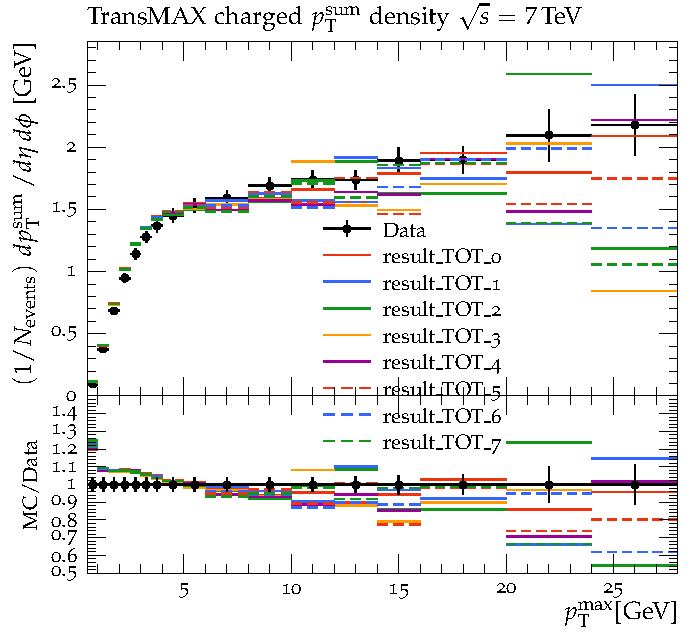
\includegraphics[width=\textwidth]{{img/Plots_2params_Finale/CMS_2012_PAS_FSQ_12_020/d08-x01-y01.pdf}}
	\end{subfigure}\\
	\begin{subfigure}{0.48\textwidth}
		\centering
		\includegraphics[width=\textwidth]{{img/Plots_2params_Finale/CMS_2012_PAS_FSQ_12_020/d06-x01-y01.pdf}}
	\end{subfigure}%
	\begin{subfigure}{0.48\textwidth}
		\centering
		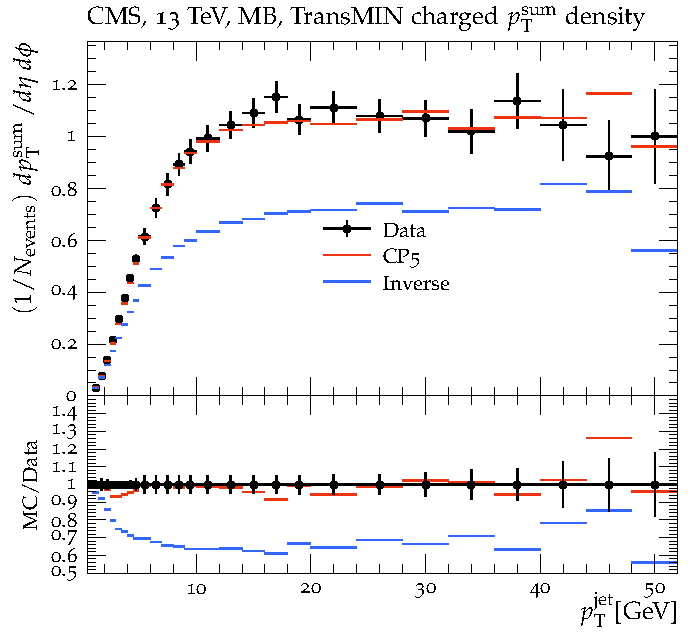
\includegraphics[width=\textwidth]{{img/Plots_2params_Finale/CMS_2012_PAS_FSQ_12_020/d09-x01-y01.pdf}}
	\end{subfigure}
	\caption{Here the data at $\sqrt{s}=7\ \mathrm{TeV}$ from the CMS analysis \cite{CMS-PAS-FSQ-12-020} for the transMAX charged particle density (upper left) and the charged $p_T$-sum (upper left); the transMIN charged particle density (lower left) and the charged $p-T$-sum are displayed as a function of the transverse momentum of the leading object.}
	\label{fig:test_2}
\end{figure}

%%%% 1.96TEV
\begin{figure}[!htb]
	\centering
	\noindent
	\begin{subfigure}{0.48\textwidth}
		\centering
		\includegraphics[width=\textwidth]{{img/Plots_2params_Finale/CDF_2015_I1388868/d01-x01-y01.pdf}}
	\end{subfigure}%
	\begin{subfigure}{0.48\textwidth}
		\centering
		\includegraphics[width=\textwidth]{{img/Plots_2params_Finale/CDF_2015_I1388868/d05-x01-y01.pdf}}
	\end{subfigure}\\
	\begin{subfigure}{0.48\textwidth}
		\centering
		\includegraphics[width=\textwidth]{{img/Plots_2params_Finale/CDF_2015_I1388868/d02-x01-y01.pdf}}
	\end{subfigure}%
	\begin{subfigure}{0.48\textwidth}
		\centering
		\includegraphics[width=\textwidth]{{img/Plots_2params_Finale/CDF_2015_I1388868/d06-x01-y01.pdf}}
	\end{subfigure}
	\caption{The transMAX charged particle density (upper left) and the charged $p_T$-sum (upper left); the transMIN charged particle density (lower left) and the charged $p-T$-sum from the CDF analysis at $\sqrt{s}=1.96\ \mathrm{TeV}$ in proton-antiproton collisions \cite{CDF:2015txs}.}
	\label{fig:test_3}
\end{figure}

\begin{figure}[!htb]
	\centering
	\includegraphics[width=0.48\textwidth]{{img/Plots_2params_Finale/CMS_2015_I1384119/d01-x01-y01.pdf}}
	\caption{In this figure is shown the last distribution we use for the tune from the CMS analysis at $\sqrt{s}=13\ \mathrm{TeV}$ \cite{CMS:2015zrm}. The pseudorapidity distribution ($|\eta|<2$) for the charged hadron density in an inelastic proton-proton scattering selection.}
	\label{fig:test_4}
\end{figure}
